\chapter{Deuteronomy 11}

\begin{figure}
  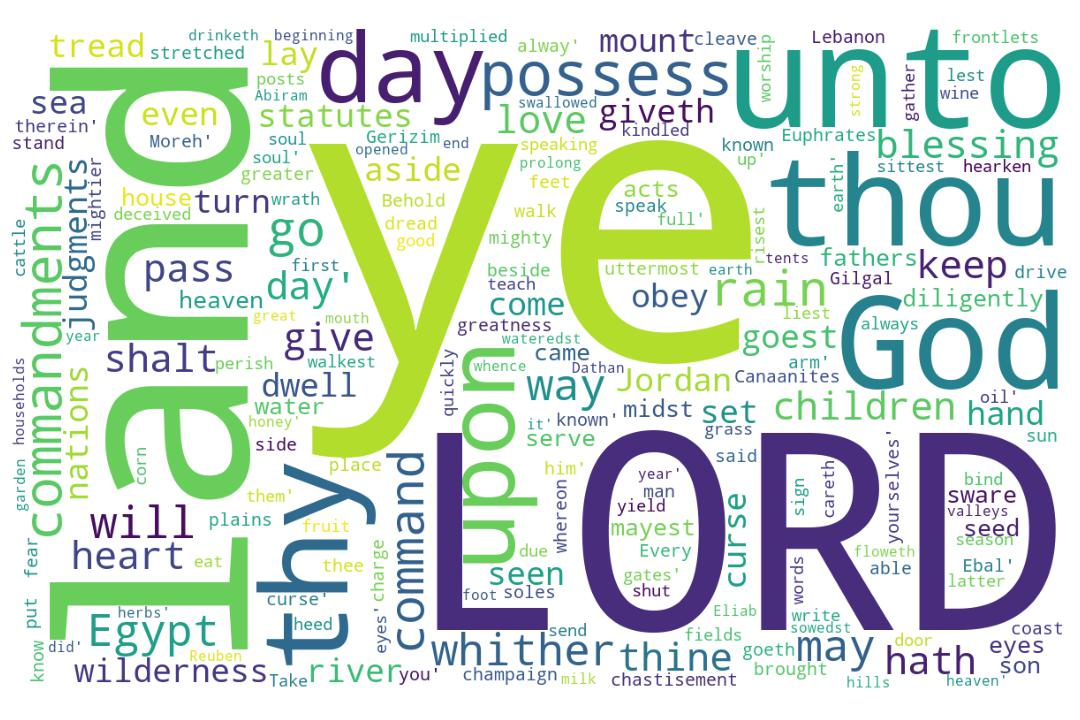
\includegraphics[width=\linewidth]{05OT-Deuteronomy/Deuteronomy11-WordCloud.jpg}
  \caption{Deuteronomy 11 Word Cloud}
  \label{fig:Deuteronomy 11 word Cloud}
\end{figure}


\marginpar{\scriptsize \centering \fcolorbox{bone}{lime}{\textbf{DECISIONS \& CONSEQUENCES}}\\ (Deuteronomy 10:1-22) \begin{compactenum}[I.][8]
    \item  God watching, from \textbf{Beginning} to the End \index[scripture]{Deuteronomy!Deu 11:12} (Deu 11:12)
    \item  \textbf{Bound} to your hands \index[scripture]{Deuteronomy!Deu 11:18} (Deu 11:26, 27, 18)
    \item  \textbf{Between} your eyes \index[scripture]{Deuteronomy!Deu 11:18} (Deu 11:26, 27, 18)
     \item  Things \textbf{Before} You\index[scripture]{Deuteronomy!Deu 11:23} \index[scripture]{Deuteronomy!Deu 11:25}\index[scripture]{Deuteronomy!Deu 11:26}\index[scripture]{Deuteronomy!Deu 11:32}(Deu 11:23, 25, 26, 32)
   \item  \textbf{Behold} -- a Choice \index[scripture]{Deuteronomy!Deu 11:26} (Deu 11:26)
    \item  \textbf{Blessings and Curses} \index[scripture]{Deuteronomy!Deu 11:26}\index[scripture]{Deuteronomy!Deu 11:27}\index[scripture]{Deuteronomy!Deu 11:29} (Deu 11:26, 27, 29)
    \item  \textbf{Brought} out and Brought in\index[scripture]{Deuteronomy!Deu 11:29} (Deu 11:26, 27, 29)
\end{compactenum}}

\footnote{\textcolor[cmyk]{0.99998,1,0,0}{\hyperlink{TOC}{Return to end of Table of Contents.}}}\footnote{\href{https://audiobible.com/bible/deuteronomy_11.html}{\textcolor[cmyk]{0.99998,1,0,0}{Deuteronomy 11 Audio}}}\textcolor[cmyk]{0.99998,1,0,0}{Therefore thou shalt love the LORD thy God, and keep his charge, and his statutes, and his judgments, and his commandments, alway.}
[2] \textcolor[cmyk]{0.99998,1,0,0}{And know ye this day: for \emph{I} \emph{speak} not with your children which have not known, and which have not seen the chastisement of the LORD your God, his greatness, his mighty hand, and his stretched out arm,}
[3] \textcolor[cmyk]{0.99998,1,0,0}{And his miracles, and his acts, which he did in the midst of Egypt unto Pharaoh the king of Egypt, and unto all his land;}
[4] \textcolor[cmyk]{0.99998,1,0,0}{And what he did unto the army of Egypt, unto their horses, and to their chariots; how he made the water of the Red sea to overflow them as they pursued after you, and \emph{how} the LORD hath destroyed them unto this day;}
[5] \textcolor[cmyk]{0.99998,1,0,0}{And what he did unto you in the wilderness, until ye came into this place;}
[6] \textcolor[cmyk]{0.99998,1,0,0}{And what he did unto Dathan and Abiram, the sons of Eliab, the son of Reuben: how the earth opened her mouth, and swallowed them up, and their households, and their tents, and all the substance that \emph{was} in their possession, in the midst of all Israel:}
[7] \textcolor[cmyk]{0.99998,1,0,0}{But your eyes have seen all the great acts of the LORD which he did.}
[8] \textcolor[cmyk]{0.99998,1,0,0}{Therefore shall ye keep all the commandments which I command you this day, that ye may be strong, and go in and possess the land, whither ye go to possess it;}
[9] \textcolor[cmyk]{0.99998,1,0,0}{And that ye may prolong \emph{your} days in the land, which the LORD sware unto your fathers to give unto them and to their seed, a land that floweth with milk and honey.}
[10] \textcolor[cmyk]{0.99998,1,0,0}{For the land, whither thou goest in to possess it, \emph{is} not as the land of Egypt, from whence ye came out, where thou sowedst thy seed, and wateredst \emph{it} with thy foot, as a garden of herbs:}
[11] \textcolor[cmyk]{0.99998,1,0,0}{But the land, whither ye go to possess it, \emph{is} a land of hills and valleys, \emph{and} drinketh water of the rain of heaven:}
[12] \textcolor[cmyk]{0.99998,1,0,0}{A land which the LORD thy God careth for: the \fcolorbox{bone}{lime}{eyes of the LORD} thy God \emph{are} always upon it, from the beginning of the year even unto the end of the year.}
[13] \textcolor[cmyk]{0.99998,1,0,0}{And it shall come to pass, if ye shall hearken diligently unto my commandments which I command you this day, to love the LORD your God, and to serve him with all your heart and with all your soul,}
[14] \textcolor[cmyk]{0.99998,1,0,0}{That I will give \emph{you} the rain of your land in his due season, the first rain and the latter rain, that thou mayest gather in thy corn, and thy wine, and thine oil.}
[15] \textcolor[cmyk]{0.99998,1,0,0}{And I will send grass in thy fields for thy cattle, that thou mayest eat and be full.}
[16] \textcolor[cmyk]{0.99998,1,0,0}{Take heed to yourselves, that your heart be not deceived, and ye turn aside, and serve other gods, and worship them;}
[17] \textcolor[cmyk]{0.99998,1,0,0}{And \emph{then} the LORD'S wrath be kindled against you, and he shut up the heaven, that there be no rain, and that the land yield not her fruit; and \emph{lest} ye perish quickly from off the good land which the LORD giveth you.}\\
\\
\P \textcolor[cmyk]{0.99998,1,0,0}{Therefore shall ye lay up these my words in your heart and in your soul, and bind them for a sign upon \fcolorbox{bone}{lime}{your hand}, that they may be as frontlets \fcolorbox{bone}{lime}{between your eyes}.}
[19] \textcolor[cmyk]{0.99998,1,0,0}{And ye shall teach them your children, speaking of them when thou sittest in thine house, and when thou walkest by the way, when thou liest down, and when thou risest up.}
[20] \textcolor[cmyk]{0.99998,1,0,0}{And thou shalt write them upon the door posts of thine house, and upon thy gates:}
[21] \textcolor[cmyk]{0.99998,1,0,0}{That your days may be multiplied, and the days of your children, in the land which the LORD sware unto your fathers to give them, as the days of heaven upon the earth.}\\
\\
\P \textcolor[cmyk]{0.99998,1,0,0}{For if ye shall diligently keep all these commandments which I command you, to do them, to love the LORD your God, to walk in all his ways, and to cleave unto him;}
[23] \textcolor[cmyk]{0.99998,1,0,0}{Then will the LORD drive out all these nations from \fcolorbox{bone}{lime}{before you}, and ye shall possess greater nations and mightier than yourselves.}
[24] \textcolor[cmyk]{0.99998,1,0,0}{Every place whereon the soles of your feet shall tread shall be your's: from the wilderness and Lebanon, from the river, the river Euphrates, even unto the uttermost sea shall your coast be.}
[25] \textcolor[cmyk]{0.99998,1,0,0}{There shall no man be able to stand before you: \emph{for} the LORD your God shall lay the fear of you and the dread of you upon all the land that ye shall tread upon, as he hath said unto you.}\\
\\
\P \textcolor[cmyk]{0.99998,1,0,0}{Behold, I set before you this day a blessing and a curse;}
[27] \textcolor[cmyk]{0.99998,1,0,0}{A blessing, if ye obey the commandments of the LORD your God, which I command you this day:}
[28] \textcolor[cmyk]{0.99998,1,0,0}{And a curse, if ye will not obey the commandments of the LORD your God, but turn aside out of the way which I command you this day, to go after other gods, which ye have not known.}
[29] \textcolor[cmyk]{0.99998,1,0,0}{And it shall come to pass, when the LORD thy God hath brought thee in unto the land whither thou goest to possess it, that thou shalt put the blessing upon mount Gerizim, and the curse upon mount Ebal.}
[30] \textcolor[cmyk]{0.99998,1,0,0}{\emph{Are} they not on the other side Jordan, by the way where the sun goeth down, in the land of the Canaanites, which dwell in the champaign over against Gilgal, beside the plains of Moreh?}
[31] \textcolor[cmyk]{0.99998,1,0,0}{For ye shall pass over Jordan to go in to possess the land which the LORD your God giveth you, and ye shall possess it, and dwell therein.}
[32] \textcolor[cmyk]{0.99998,1,0,0}{And ye shall observe to do all the statutes and judgments which I set before you this day.}